% Драфт секции: Вовлечённость отдельных нейронов в популяционный код (NOF)
% Корректная версия (после deep-analysis по метрике реконструкции).
% Основной код — автокодировщик (AE, lambda=0); PCA/UMAP — контроль (sanity check).
% Меры: значимость связи нейрон-код (MI/INTENSE) + градуированная (ранговая корреляция).
% Фигуры: images/popcode/fig_popcode_geometry.png, fig_popcode_involvement.png
% Данные/скрипты: drafts/ch3/popcode/ (involvement_v3, space_coding_compare)
% Статус: черновик для ревью; в основной текст не внесён.

\section{Вовлечённость отдельных нейронов в популяционный код}\label{sec:popcode}

\link{Связка: предыдущие главы рассматривали два уровня описания нейронной активности по отдельности~--- популяционный (геометрия коллективных переменных, секции~\ref{sec:dim}, \ref{sec:v2}) и индивидуальный (селективность отдельных нейронов, секция~\ref{sec:intense}). Оба опираются на одни и те же записи, поэтому естественно поставить вопрос об их связи: тот же информационно-теоретический критерий, что выявляет селективность к поведению, применим и к коллективным переменным.}

Анализ соотношения популяционного и индивидуального кодирования важен для понимания вычислительной роли коллективной активности. Согласно гипотезе лог-динамического мозга~\cite{Buzsaki2014}, лишь малая доля нейронов обладает сильными устойчивыми специализациями. Остаётся открытым, как эта неоднородность связана с популяционным кодом: формируют ли поведенчески селективные нейроны его преимущественно или код поддерживается широкой смесью клеток. Метод INTENSE (секция~\ref{sec:intense}) позволяет поставить этот вопрос количественно, рассматривая коллективную переменную как ещё одну динамическую величину.

\subsection{Коллективные переменные и меры вовлечённости}\label{sec:popcode_method}

Коллективная активность популяции в каждый момент времени описывается небольшим набором \emph{коллективных переменных}~--- низкоразмерных координат, обобщающих совместную динамику всех зарегистрированных нейронов. Их извлекали снижением размерности: основным представлением служил автокодировщик (16-мерный код, обучаемый восстанавливать активность всей популяции), а метод главных компонент (PCA) и UMAP использовались как контрольные представления~--- чтобы убедиться, что вывод не зависит от способа извлечения кода. Все вычисления выполнены средствами пакета DRIADA (секция~\ref{sec:driada}).

\emph{Вовлечённость} нейрона в коллективный код отражает, в какой мере его активность подчинена коллективной динамике популяции, а не разворачивается независимо от неё. Мы оценивали её двумя взаимодополняющими способами. Во-первых, проверялось \textit{наличие} связи: значимая (метод INTENSE, секция~\ref{sec:intense}) взаимная информация между активностью нейрона и коллективной переменной означает, что нейрон несёт информацию о коллективном состоянии популяции. Во-вторых, оценивалась \textit{сила} вовлечённости~--- насколько коллективное состояние популяции предсказывает активность самого нейрона.

Силу оценивали следующим образом. Пусть $Z(t)\in\mathbb{R}^{16}$~--- коллективное состояние популяции в момент $t = 1,\dots,T$, а $x_n(t)$~--- активность нейрона $n$. Активность нейрона предсказывали из коллективного состояния по принципу <<когда популяция находилась в близком состоянии, что в среднем делал этот нейрон>>: усредняли активность нейрона по $k = 10$ моментам, ближайшим к $Z(t)$ в пространстве коллективных переменных,
\begin{equation}
\hat{x}_n(t) = \frac{1}{k}\sum_{\tau\,\in\,\mathcal{N}_k(t)} x_n(\tau),
\label{eq:knn_pred}
\end{equation}
где $\mathcal{N}_k(t)$~--- $k$ ближайших к $Z(t)$ моментов обучающей выборки. Вовлечённость нейрона~--- ранговая корреляция (Спирмена) между этим предсказанием и реальной активностью: она высока, если разряды нейрона воспроизводятся коллективным состоянием популяции, и близка к нулю, если активность нейрона от коллективной динамики не зависит.

Несколько предосторожностей обеспечивают корректность оценки. Совпадение предсказания с реальной активностью измерялось корреляцией, а не долей объяснённой дисперсии: кальциевый сигнал состоит из редких импульсов, и доля дисперсии отражала бы в основном точность воспроизведения их амплитуды, недооценивая совпадение самого паттерна активности. Обучающие и проверочные моменты разделялись непрерывными временны́ми блоками (пять блоков), а не случайно: иначе активность нейрона предсказывалась бы по соседним во времени кадрам, и медленная динамика кальциевого индикатора завышала бы оценку. Наконец, вовлечённость оценивалась по коду как целому, а не по отдельным его компонентам. Шестнадцать коллективных переменных совместно описывают состояние популяции, но их разбиение на отдельные оси произвольно: то же состояние можно равноценно задать другим, <<повёрнутым>> набором из шестнадцати переменных. Поэтому утверждение <<нейрон связан с компонентой №3>> зависит от того, как именно проведены оси, и не является свойством самого нейрона; биологический смысл имеет лишь его связь с коллективным состоянием популяции в целом.

Поведенческая селективность тех же нейронов бралась из анализа INTENSE по поведенческим переменным (положение, скорость, направление движения, заходы в зоны арены и т.п.; секция~\ref{sec:intense}). Анализировались 64 сессии (16 мышей по четыре дня; секция~\ref{sec:nof_data}). Все статистические сравнения проводились на уровне животных ($n=16$): показатели усреднялись по дням каждой мыши, поскольку четыре сессии одной мыши не являются независимыми наблюдениями.

\subsection{Восстановление геометрии среды}\label{sec:popcode_geometry}

Коллективный код восстанавливает пространственное положение животного. Двумерная проекция кода, окрашенная двумерной цветовой картой положения, обнаруживает согласованный пространственный градиент (рис.~\ref{fig:popcode_geom}A): близкие в коде состояния соответствуют близким положениям. Количественно положение декодируется из кода с ошибкой около $9{,}4 \pm 1{,}1$~см при стороне арены 44~см; автокодировщиковый код точнее, чем PCA и UMAP (парный критерий Уилкоксона по животным, $p < 0{,}01$), и все три кода значимо точнее случайного уровня ($p < 10^{-4}$; рис.~\ref{fig:popcode_geom}B). Это согласуется с результатами секций~\ref{sec:dim} и~\ref{sec:v2} и распространяет их на реконструкционный код.

\begin{figure}[ht]
\centering
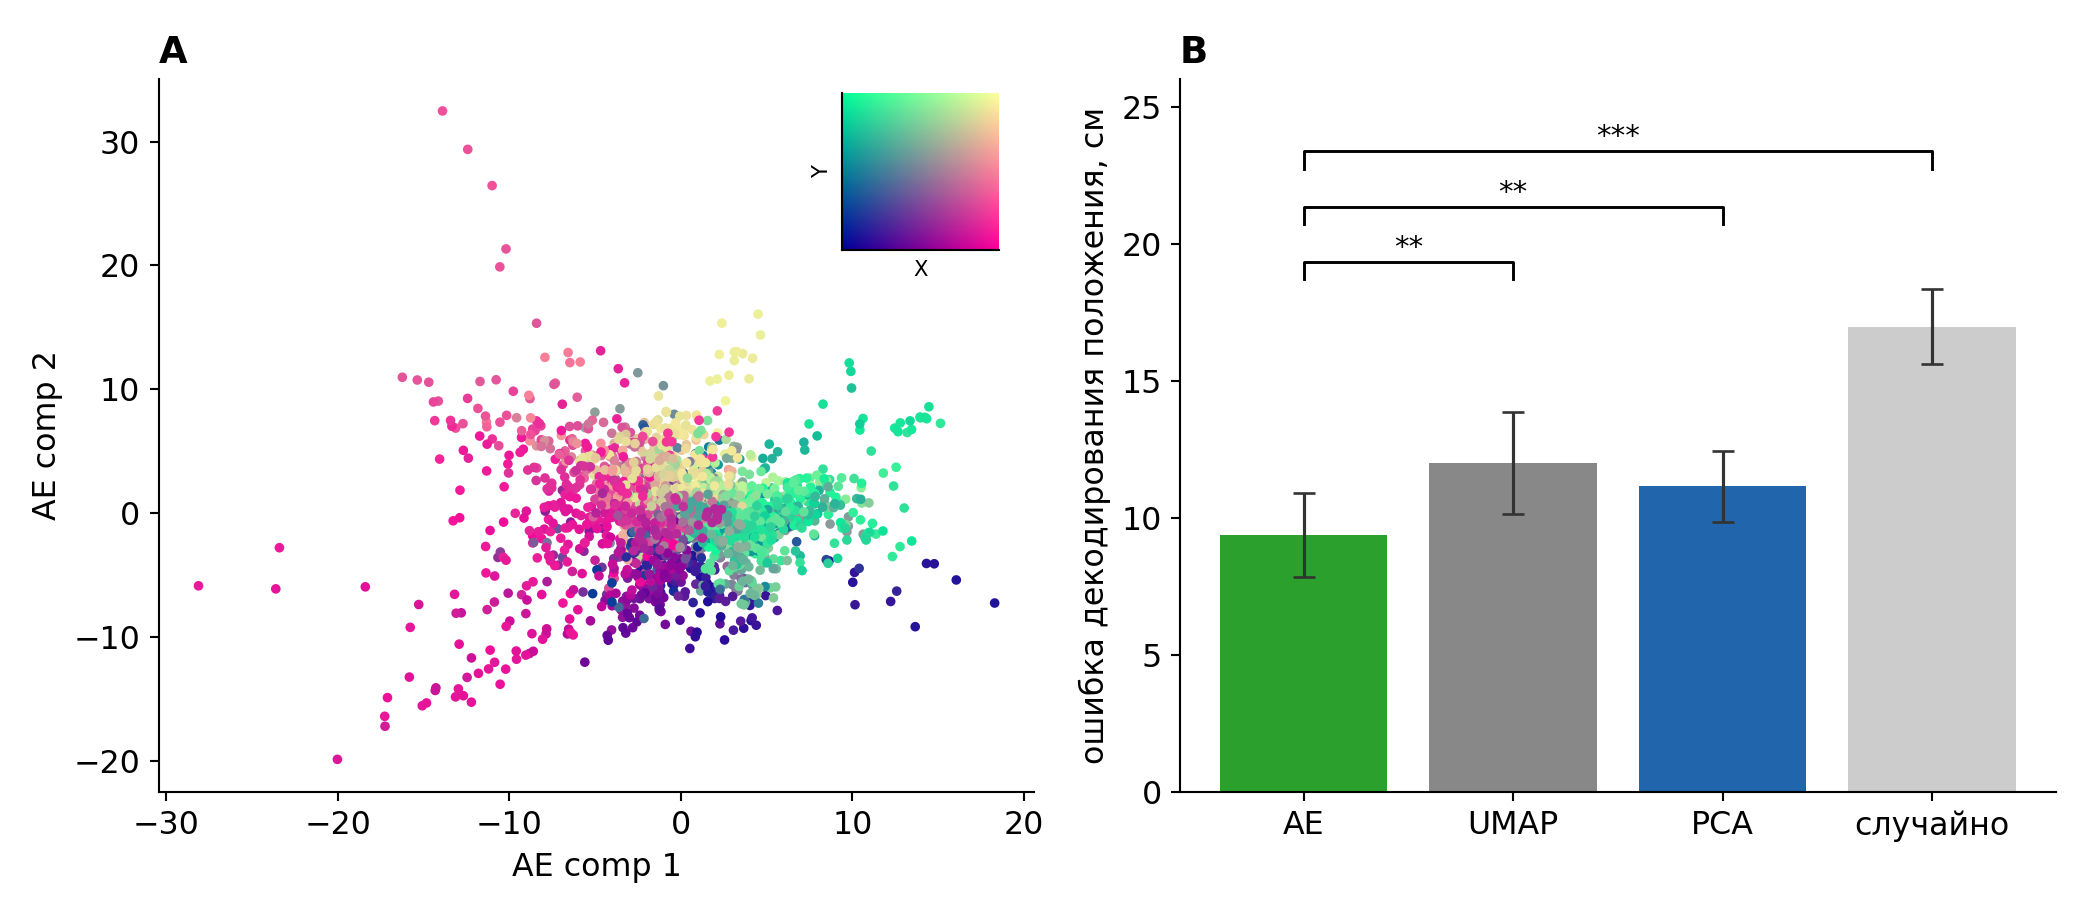
\includegraphics[width=0.95\textwidth]{images/popcode/fig_popcode_geometry.png}
\caption{Восстановление геометрии среды коллективным кодом. \textbf{A}~--- двумерная проекция автокодировщикового кода (одна сессия); цвет кодирует положение животного двумерной картой (вставка: оси $X$, $Y$). \textbf{B}~--- ошибка декодирования положения методом $k$ ближайших соседей (кросс-валидация по непрерывным временны́м интервалам; среднее $\pm$ 95\,\% доверительный интервал по 16 животным). Все сравнения~--- парный критерий Уилкоксона на уровне животных ($n=16$). Автокодировщик (AE) точнее PCA и UMAP ($p<0{,}01$) и значимо ниже случайного уровня ($p<10^{-4}$).}
\label{fig:popcode_geom}
\end{figure}

\subsection{Вовлечённость и её связь с поведением}\label{sec:popcode_involvement}

Применённый покомпонентно, метод INTENSE помечает значимой связь хотя бы с одной коллективной переменной у $59 \pm 9\,\%$ нейронов (среднее по животным; от 25 до 94\,\% по отдельным сессиям). Однако отдельные компоненты кода не имеют самостоятельного смысла: те же шестнадцать коллективных переменных можно задать другим, <<повёрнутым>> набором, и тогда то, к какой компоненте и скольким из них <<селективен>> нейрон, изменится. Поэтому покомпонентная доля зависит от того, как проведены оси, и не является свойством нейрона. Поэтому вовлечённость характеризуется на уровне кода как целого: положительную корреляцию восстановления активности из всего кода имеют около 92\,\% нейронов (рис.~\ref{fig:popcode_inv}C). Сила вовлечённости при этом умеренная (медианная ранговая корреляция около $0{,}15$) и убывает с ростом числа зарегистрированных нейронов: низкоразмерный код удерживает общую структуру популяции, тогда как значительная часть активности отдельного нейрона приватна и из кода не восстанавливается. Распределения вовлечённости для автокодировщика, PCA и UMAP близки (рис.~\ref{fig:popcode_inv}C), то есть вывод не является артефактом конкретного метода.

Связь вовлечённости с поведенческой селективностью~--- умеренно положительная. Вовлечённость поведенчески селективных нейронов выше, чем неселективных ($0{,}21$ против $0{,}16$; $p = 3{,}1\cdot10^{-5}$, парный критерий Уилкоксона по животным; рис.~\ref{fig:popcode_inv}A), а ранговая корреляция вовлечённости с поведенческой взаимной информацией нейрона составляет $\rho \approx 0{,}28$ (значимость оценена по корреляциям, усреднённым по 16 животным, $p = 3{,}1\cdot10^{-5}$; рис.~\ref{fig:popcode_inv}B). Это существенно слабее, чем преимущественное участие селективных нейронов: код опирается на широкую смесь поведенчески селективных и неселективных клеток.

\begin{figure}[ht]
\centering
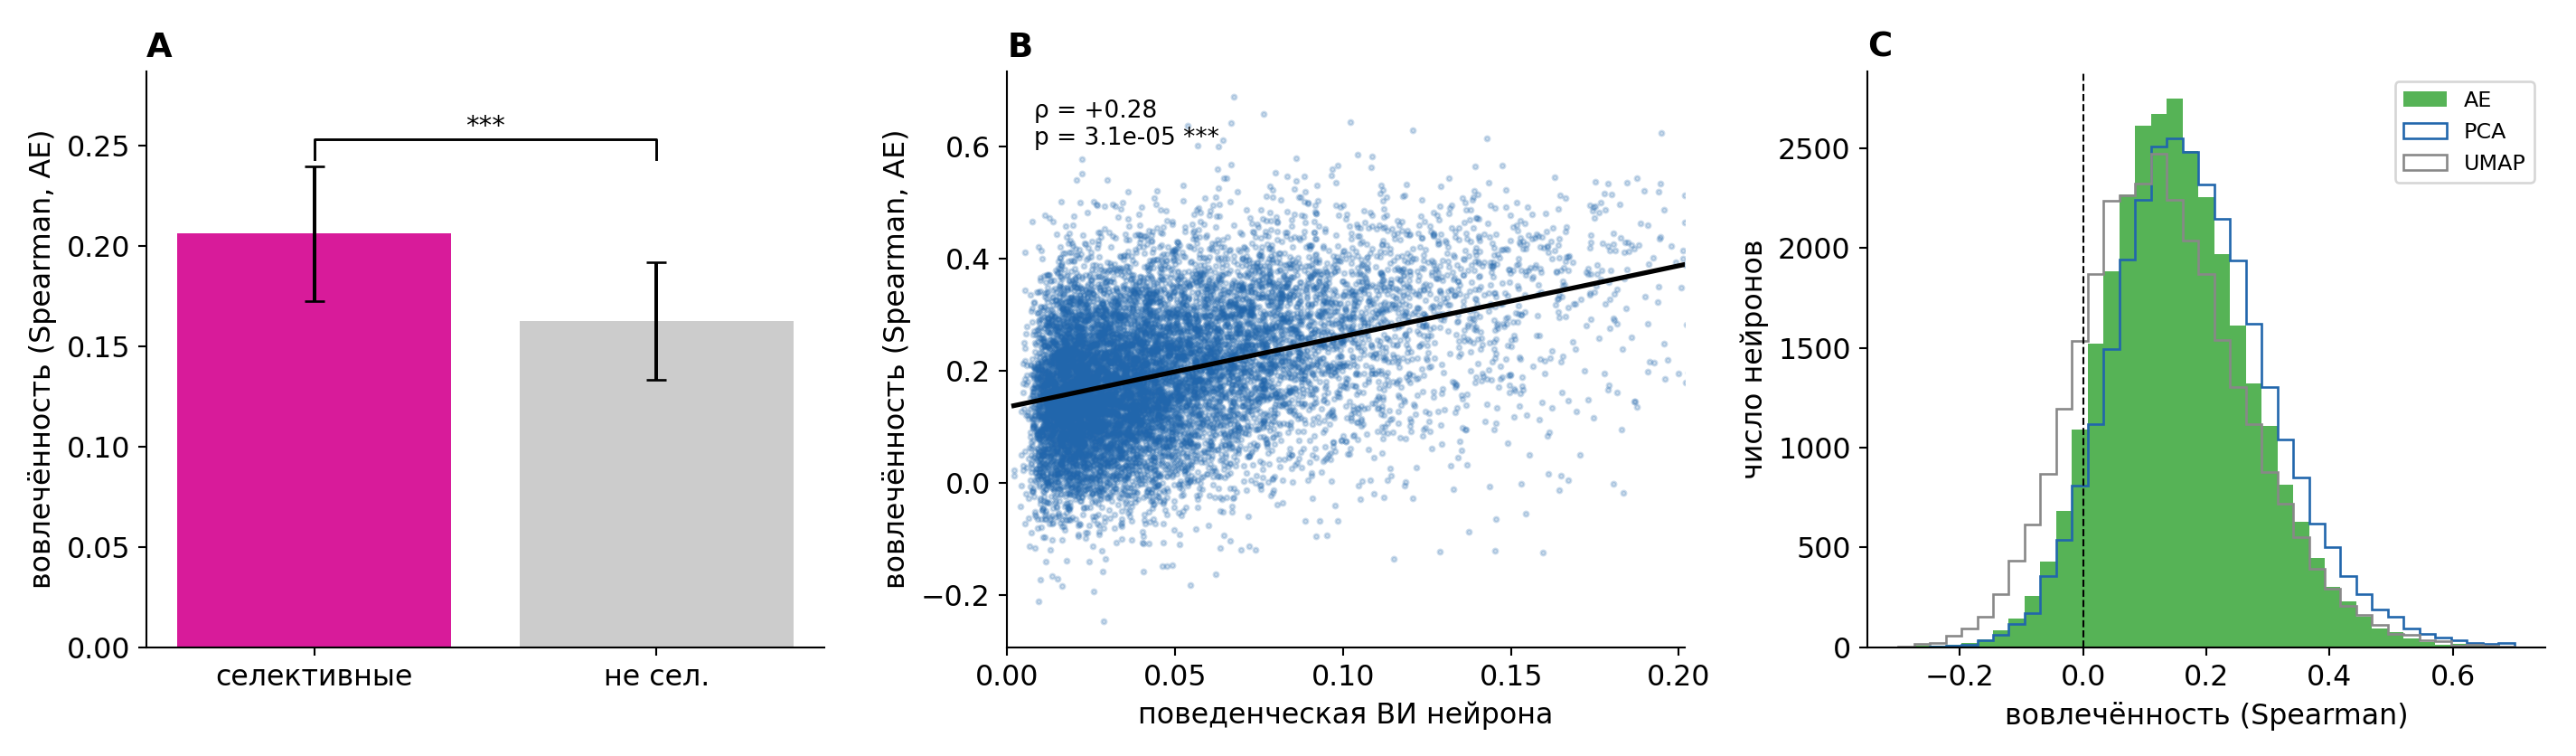
\includegraphics[width=0.98\textwidth]{images/popcode/fig_popcode_involvement.png}
\caption{Вовлечённость нейронов в коллективный код и её связь с поведением (64 сессии; вовлечённость~--- ранговая корреляция предсказанной и истинной активности при блочной кросс-валидации). Все сравнения~--- на уровне животных ($n=16$). \textbf{A}~--- вовлечённость поведенчески селективных нейронов выше, чем неселективных (парный критерий Уилкоксона, $p = 3{,}1\cdot10^{-5}$; среднее $\pm$ 95\,\% доверительный интервал по животным). \textbf{B}~--- связь вовлечённости с поведенческой взаимной информацией нейрона; чёрная линия~--- линейная аппроксимация; значимость тренда оценена по ранговым корреляциям, усреднённым по 16 животным ($\rho = 0{,}28$, $p = 3{,}1\cdot10^{-5}$). \textbf{C}~--- распределение вовлечённости: автокодировщик~--- заливкой, PCA и UMAP~--- контуром (контроль); положительна у $\sim$92\,\% нейронов.}
\label{fig:popcode_inv}
\end{figure}

\subsection{Обсуждение}\label{sec:popcode_discussion}

Полученная картина соответствует сильно распределённому коду: в формирование коллективных переменных вовлечена почти вся популяция, но вклад каждого отдельного нейрона умеренный, и выделенного <<ядра>> сильно вовлечённых клеток не наблюдается. Поведенческая селективность нейрона слабо положительно связана с его вовлечённостью, но не определяет её: коллективный код поддерживается смесью селективных и неселективных клеток. Это уточняет более ранние оценки преимущественного участия поведенчески значимых нейронов, которые, по-видимому, отражали меньшую чувствительность прежнего анализа селективности.

Методологически важно, что вовлечённость корректно определена лишь на уровне кода в целом. Отдельные оси автокодировщикового или UMAP-представления можно произвольно <<повернуть>>, не меняя описания популяции, поэтому связь нейрона с конкретной осью не является его свойством; устойчивы (не зависят от выбора осей) лишь характеристики, относящиеся ко всему коду~--- значимость связи с ним и качество восстановления активности нейрона. Тот же информационно-теоретический критерий, что выявляет селективность к поведению (секция~\ref{sec:intense}), связывает индивидуальный и популяционный уровни в единой схеме; его субстрат-независимость подтверждается применением к импульсной сети (секция~\ref{sec:mango}), где per-neuron взаимная информация сопоставлялась с вкладом нейронов в популяционные характеристики.
